\documentclass{beamer}
\usepackage{graphicx}
\usepackage{caption}
\usepackage{subcaption}
\usepackage{color}
\usepackage{listings}
\usepackage{verbatim}
\captionsetup{compatibility=false}
%\usepackage[italian]{babel}  

%% Se per qualsiasi motivo non riuscissi a compilare col tema Unipd,
%% basta commentare la riga qui sotto e si passa automaticamente al
%% tema beamer di default.
\usetheme{Unipd}

\lstdefinestyle{customc}{
  belowcaptionskip=1\baselineskip,
  breaklines=true,
  %frame=L,
  xleftmargin=\parindent,
  language=C,
  showstringspaces=false,
  basicstyle=\fontsize{7}{7}\selectfont\ttfamily,%\footnotesize\ttfamily,
  keywordstyle=\bfseries\color{green!40!black},
  commentstyle=\itshape\color{gray},
  identifierstyle=\color{blue!40!black},
  %stringstyle=\color{orange},
}
\lstset{escapechar=@,style=customc}

\title{Continuous Integration}
%\subtitle{da inserire}
\author{Diego Casella}
\date{\today}

\begin{document}

\maketitle

\begin{frame}{Contenuti} %Outline
\tableofcontents
\end{frame}

%% Introduzione
\section{Introduzione}
\begin{frame}{Introduzione}
In questo seminario affronteremo la pratica della Continuous Integration: introdurremo le motivazioni che hanno portato alla sua formalizzazione, i princ\'ipi sui quali essa si fonda, e come venga applicata nella pratica
\end{frame}

\section{Cos'\'e la Continuous Integration}
\begin{frame}{Cos'\'e la Continuous Integration}
Il concetto di \emph{Continuous Integration}, di seguito abbreviata con \textbf{CI}, \'e una pratica nata dall'\emph{extreme programming} e successivamente sviluppatasi in maniera autonoma, che si applica nei contesti in cui lo sviluppo software avviene attraverso un sistema di versioning.
\newline
Essa si propone come una tecnica complementare al \emph{Test Driven Development}, dove infatti si suppone che esistano
sistemi di test automatici, che i vari programmatori possano esegurie prima di pubblicare le loro modifiche nel server centrale.
\end{frame}


\subsection{Origini della Continuous Integration}
\begin{frame}{Origini della \textbf{CI}}
Si consideri il seguente scenario:
\begin{itemize}
\item una azienda software composta da venti sviluppatori;
\item ogni sviluppatore lavora alla propria postazione, clonando il codice dal repository centrale;
\item le nuove feature o fix vengono inviate al repository centrale	quando sono state realizzate (dopo \emph{''x''} ore, giorni, settimane?);
\end{itemize}
\end{frame}


\begin{frame}{Origini della \textbf{CI} (2)}
Questo scenario \'e critico per le seguenti ragioni:
\begin{itemize}
\item ogni volta che un repository viene clonato, ed uno sviluppatore inizia a lavorare in esso, tale clone si disallinea con lo stato del repository centrale;
\item tale differenza si accresce in maniera proporzionale al tempo impiegato dallo sviluppatore per il suo lavoro;
\end{itemize}
\end{frame}


\begin{frame}{Origini della \textbf{CI} (3)}
Questo scenario \'e critico per le seguenti ragioni:
\begin{itemize}
\item quando uno sviluppatore vuole pubblicare le proprie modifiche, incorre in un possibile conflitto dovuto ad altri commit realizzati dai suoi colleghi. Tale rischio aumenta con l'aumentare del tempo trascorso fra un proprio commit, e quello successivo;
\item si raggiunge un punto per cui il tempo impiegato per integrare le modifiche altrui, eguaglia o addirittura supera il tempo speso per realizzare le proprie.
\end{itemize}
\end{frame}


\begin{frame}{Origini della \textbf{CI} (4)}
Questo scenario \'e critico per le seguenti ragioni:
Si viene dunque a configurare una situazione estremamente negativa per l'attivit\'a di sviluppo del programmatore e
del ciclo di vita software stesso, che viene comunemente denominata \emph{integration/merge hell}.
\newline
Ecco quindi che entra in gioco la \textbf{CI}, con lo scopo di mitigare notevolmente gli effetti negativi dello sviluppo di un
software da parte di pi\'u entit\'a.
\end{frame}


\section{Princ\'ipi della Continuous Integration}
\begin{frame}{Princ\'ipi della \textbf{CI}}
\begin{block}{Gestione del codice tramite version control}
La pratica del \textbf{CI} impone che il codice sia sotto versioning, e lo stesso vale anche per eventuali script, file di
configurazione e di build che sono necessari per effettuare una build del programma. Inoltre ci si aspetta che, dopo un checkout
dal repository, il codice sorgente sia compilabile ed eseguibile senza errori.
\end{block}
\end{frame}

\begin{frame}{Princ\'ipi della \textbf{CI}}
\begin{block}{Automatizzazione della build}
Per \emph{build} si intende il senso pi\'u ampio del termine, ovvero:
\begin{itemize}
\item rendere automatica l'operazione di compilazione del codice sorgente;
\item rendere automatica la generazione della documentazione, pagine web, pacchetti di deploy e diagnostica finale;
\end{itemize}
il tutto ovviamente senza l'intervento diretto dello sviluppatore.
\end{block}
\end{frame}

\begin{frame}{Princ\'ipi della \textbf{CI}}
\begin{block}{Rendere la build self-testing}
Ogni qual volta viene effettuata una nuova build, devono essere eseguiti tutti i test presenti nel codice. Ci\'o assicura che le 
modifiche fatte si comportino come nei test scritti in precedenza, senza generare errori.
\end{block}
\end{frame}

\begin{frame}{Princ\'ipi della \textbf{CI}}
\begin{block}{Committare nel repository centrale ogni giorno}
Committando regolarmente, ogni sviluppatore riduce il rischio di conflitti complessi da risolvere. Inoltre, la risoluzione di questi
conflitti ''minori'' produce l'effetto di tenere costantemente aggiornati ogni membro del gruppo sul lavoro svolto dagli altri.
svolto dagli altri
\end{block}
\end{frame}

\begin{frame}{Princ\'ipi della \textbf{CI}}
\begin{block}{Ogni commit innesca un processo di build}
Ogni volta che si effettua un commit nel \textbf{repository centrale} (svn vs. git), il server stesso deve lanciare una build dell'applicazione per poter determinare l'integrit\'a del codice inviatogli. Se il
l'operazione non \'e andata a buon termine, l'errore va corretto immediatamente.
\end{block}
\end{frame}

\begin{frame}{Princ\'ipi della \textbf{CI}}
\begin{block}{Il processo di build deve essere veloce}
Dato che ogni commit deve essere compilato dal server, \'e necessario che questa operazione sia veloce per permettere a tutti
gli sviluppatori di inviare il proprio codice senza aspettare che il server termini la build precedente. Questo principio, perch\'e
sia efficace, si basa a sua volta sulla premessa che il software sia \emph{modulare} e che dunque sia necessario, di volta involta,
ricompilare solo una piccola parte di esso per poter verificare l'integrit\'a del suo complesso.
\newline
\'E bene inoltre pianificare delle \emph{nightly build}, che effettuino build da zero, verificandone di nuovo l'integrit\'a complessiva
ed eseguendo i test presenti.
\end{block}
\end{frame}

\begin{frame}{Princ\'ipi della \textbf{CI}}
\begin{block}{Eseguire i test in un clone dell'ambiente di produzione}
Se l'ambiente su cui vengono eseguiti i test non \'e assolutamente identico all'ambiente di produzione, c'\'e il rischio che qualcosa
che \'e stato testato generi dei bug inspiegabili una volta rilasciato in produzione, con conseguenti danni economici e di immagine.
\end{block}
\end{frame}

\begin{frame}{Princ\'ipi della \textbf{CI}}
\begin{block}{Semplificare l'ottenimento delle ultime versioni dei pacchetti software}
Rendere le ultime versioni disponibili ai clienti o ai tester, riduce il rischio di introdurre funzionalit\'a che non corrispondono a
quanto il cliente si aspetta. Di conseguenza si pu\'o agire prima e pi\'u efficacemente per correggere il proprio prodotto.
\end{block}
\end{frame}

\begin{frame}{Princ\'ipi della \textbf{CI}}
\begin{block}{Tutti possono vedere i risultati delle ultime build}
Ci\'o \'e necessario per accorgersi il prima possibile se una build non compila, o sono stati generati errori nei test associati, e
dunque sistemarli prima che tali modifiche vengano scaricate dagli altri membri del team di sviluppo.
\end{block}
\end{frame}

\begin{frame}{Princ\'ipi della \textbf{CI}}
\begin{block}{Automatizzare il deploy}
Molti software di \textbf{CI} forniscono anche la funzionalit\'a di deploy su di un test server al quale tutti gli sviluppatori hanno
accesso per poter effettuare altri controlli pu\' affinati con l'ultima build disponibile.
\end{block}
\end{frame}

\begin{frame}{Princ\'ipi della \textbf{CI}}
Anche se tutto ci\'o pu\'o sembrare rindondante e macchinoso, i benefici che si ottengono sono molteplici:
\begin{itemize}
\item i bug di integrazione vengono scovati molto presto e, dato che le modifiche sono contenute, \'e piu\' semplice risolverli,
facendo risparmiare tempo e denaro;
\item si elimina il caos pre-release, dove tutti cercano di integrare il risultato di giorni, se non settimane, di lavoro;
\item disponibilit\'a costante di una build corrente che pu\'o essere utilizzata per scopi di testing, demo o release;
\item i costanti check eseguiti sul software spronano gli sviluppatori a creare codice organizzato e modulare;
\end{itemize}
\end{frame}


\section{Software per la Continuous Integration}
\begin{frame}{Software per la Continuous Integration}
Ora che conosciamo princ\'ipi cardine che costituiscono la \textbf{CI}, descriveremo brevemente i software pi\'u utilizzati nel
campo vedendone i principali pregi e difetti. Prima di fare ci\'o, le caratteristiche che li accomunano sono:
\begin{itemize}
\item una interfaccia per configurare il software stesso, solitamente esposta tramite browser web (certi forniscono anche una gui
standalone);
\item analisi statica del codice, con tanto di raccolta di statistiche sulla qualit\'a del codice presente;
\item integrazione con i (D)VCS maggiormente utlizzati come ad esempio git, svn, bazaar, mercurial, perforce ecc...;
\item RSS, invio automatico di email in caso di build errata;
\item esecuzione di script customizzati;
\end{itemize}
\end{frame}


\subsection{Cruise Control}
\begin{frame}{Cruise Control}
Cruise Control \'e uno dei pi\'u vecchi  software per \textbf{CI}. \'E stato sviluppato da Kent Beck e Ron Jeffries, coloro 
che hanno coniato il termine \emph{Extreme Programmig}, definendone i princ\'ipi base.
\begin{figure}
  \centering
  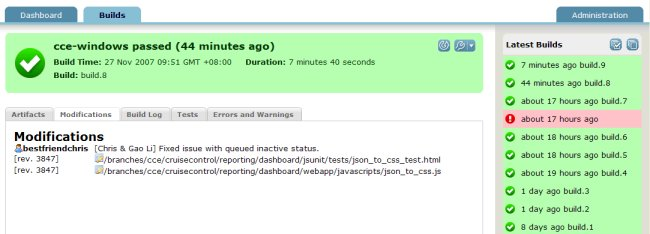
\includegraphics[scale=0.4]{images/cruise_control.jpg}
  \caption{Cruise Control Web Interface}
\end{figure}
\end{frame}


\begin{frame}{Cruise Control - Caratteristiche}
\'E stato ideato specificatamente per progetti realizzati in Java, anche se esiste una versione denominata \emph{Cruise Control
.Net} che \'e indirizzata al linguaggio .Net, e una versione \emph{Cruise Control.rb} per linguaggio Ruby . Non presenta una gui
per configurarlo: l'intero processo avviene tramite scrittura di un file xml a mano, anche se esistono dei tool di terze parti che
facilitano tale setup. Possiede una web UI molto primitiva, e la curva d'apprendimento \'e molto ripida; tuttavia, una volta
installato e configurato opportunamente, si dimostra molto affidabile.
\end{frame}


\begin{frame}{Cruise Control - Caratteristiche}
\begin{figure}
  \centering
  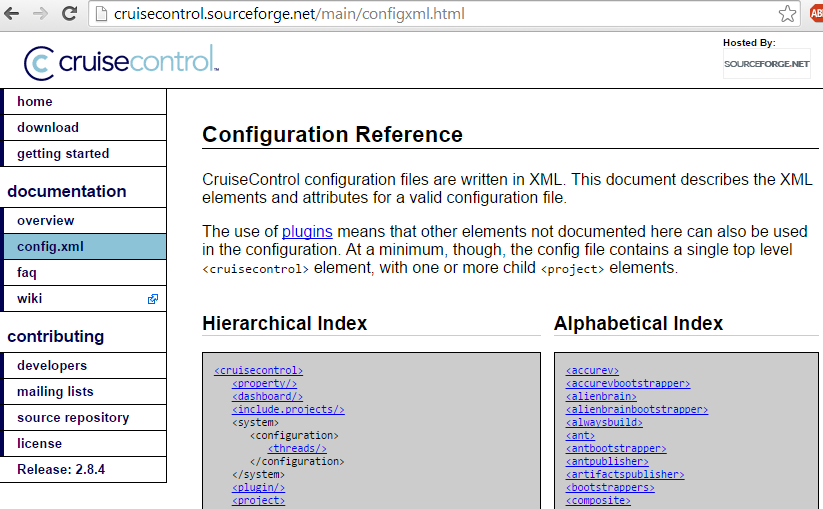
\includegraphics[scale=0.4]{images/cruise_control_cfg.jpg}
  \caption{XML configuration API}
\end{figure}
\end{frame}


\begin{frame}{Cruise Control - Caratteristiche}
Cruise Contro \'e disponibile per qualsiasi tipo di piattaforma, dispone di builders sia per Ant che Maven, dispone di un sistema di
 notifica tramite email e CCTray, ed \'e presente un plugin per l'integrazione con Eclipse.
\newline \'E rilasciato sotto licenza BSD.
\end{frame}


\subsection{Jenkins}
\begin{frame}{Jenkins}
Jenkins si \'e fatto largo negli anni come il software per \textbf{CI} nell'ambito di progetti opensource. \'E nato da un fork del
progetto Hudson, sviluppato da Oracle, e si \'e inseguito sviluppato indipendentemente ed in chiaro, raggiungendo il numero di
ben 567 project members (contro i 32 di Hudson).
\newline
Jenkins si contraddistingue per una elevata configurabilit\'a e semplicit\'a di utilizzo, unita ad una web interface molto funzionale.
\end{frame}


\begin{frame}{Jenkins - Caratteristiche}
\begin{figure}
  \centering
  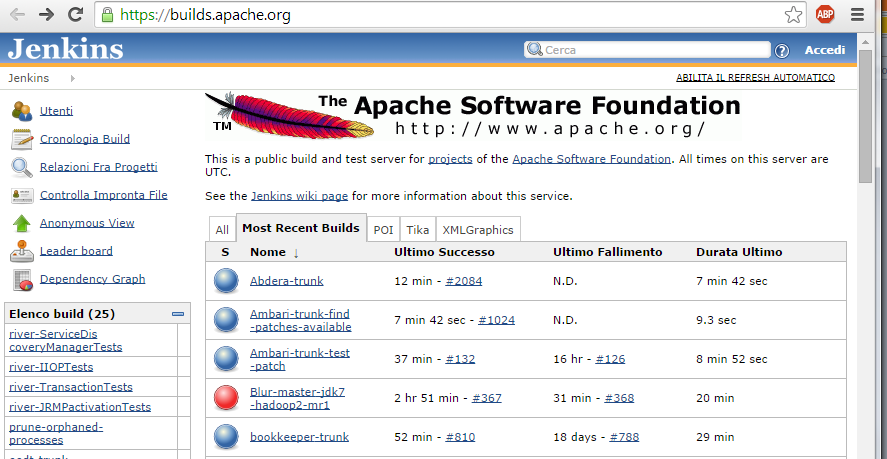
\includegraphics[scale=0.35]{images/jenkins.png}
  \caption{Jenkins Web Interface}
\end{figure}
\end{frame}


\begin{frame}{Jenkins - Caratteristiche}
Jenkins \'e funzionante come Java servlet, e dunque \'e installabile in qualsiasi macchina che abbia presente una JVM; dispone
di builders  MSBuild, Ant e Maven, CMake, Grails, Ruby, Scons, Python e molti altri ancora. Integra inoltre sistemi di notifica
tramite email, RSS, Google Calendar, bot IRC, XMPP e twitter, ed \'e integrato attraverso plugin per Eclipse, NetBeans ed 
IntelliJ IDEA. Inoltre \'e anche integrato con software per il bug tracking quali Bugzilla, Google Code, JIRA, Redmine ed altri
ancora. \'E licenziato secondo la Creative Commons e MIT License.
\end{frame}


\subsection{Apache Continuum}
\begin{frame}{Apache Continuum}
Apache Continuum \'e funzionante, come Jenkins/Hudson, attraverso un Servlet Java. Tuttavia, non supporta Windows builders,
e per quanto riguarda Java, \'e disponibile solo Maven. Prevede l'invio di notifiche tramite email, Jabber e Google Talk, MSN ed
IRC. Al momento, non si conoscono integrazioni con gli IDE pi\'u diffusi, n\'e con sistemi di bugtracking.
\end{frame}


\begin{frame}{Apache Continuum}
\begin{figure}
  \centering
  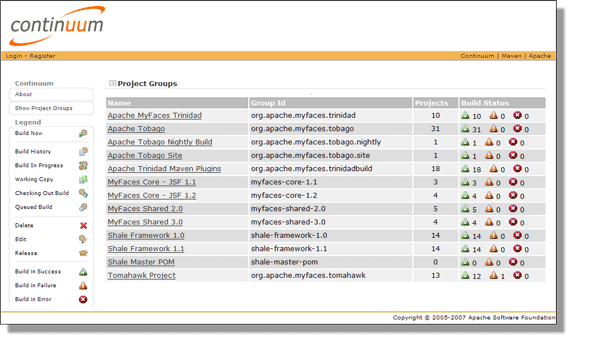
\includegraphics[scale=0.35]{images/apache_continuum.png}
  \caption{Apache Continuum Web Interface}
\end{figure}
\end{frame}


\subsection{Apache Gump}
\begin{frame}{Apache Gump}
Apache Gump \'e stato il primo sistema di \textbf{CI} realizzato da Apache. \'E scritto interamente in Python, e dunque funziona
in qualsiasi macchina dotata di un suo interpete. Gli unici builders che supporta sono Ant e Maven (solo versione 1, la e 3 no)
e l'unico mezzo di notifica \'e tramite email. Non \'e integratoi con IDE o sistemi di bugtracking. 
\end{frame}


\begin{frame}{Apache Gump}
\begin{figure}
  \centering
  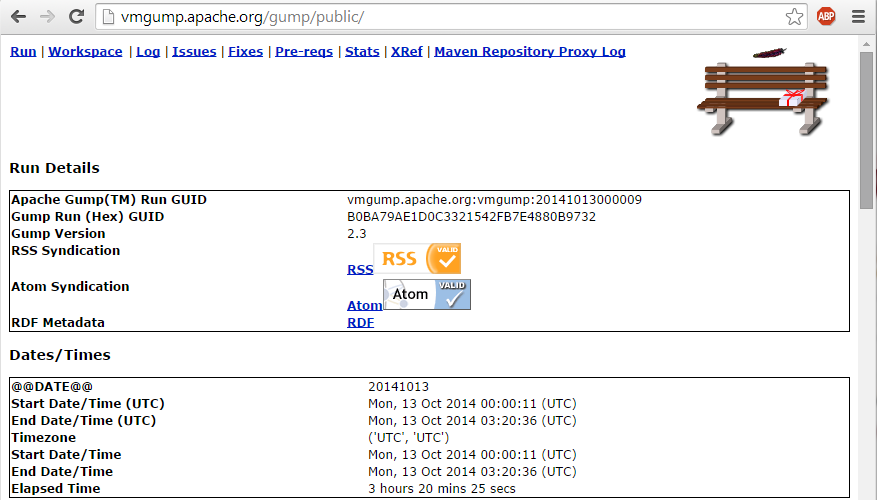
\includegraphics[scale=0.35]{images/apache_gump.png}
  \caption{Apache Gump Web Interface}
\end{figure}
\end{frame}


\begin{frame}{Apache Gump}
\begin{figure}
  \centering
  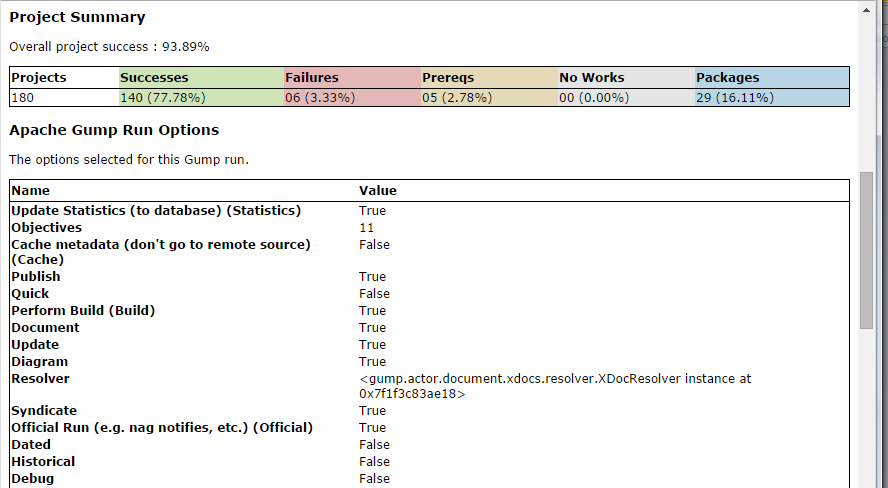
\includegraphics[scale=0.35]{images/apache_gump2.png}
  \caption{Apache Gump Web Interface}
\end{figure}
\end{frame}

\section{Q\&A}
\begin{frame}{Q\&A}
\end{frame}

\end{document}
